\documentclass[11pt]{report}
\usepackage{fullpage}
\usepackage{graphicx}

\title{\bf {\Huge Design Patterns}\\
\huge Elements of Reusable Object-Oriented Software}
\author{Gang of Four}
\date{}
\usepackage{color}
\usepackage{listings}
\lstset{ %
language=C++,                % choose the language of the code
basicstyle=\small,       % the size of the fonts that are used for the code
numbers=left,                   % where to put the line-numbers
numberstyle=\scriptsize,      % the size of the fonts that are used for the line-numbers
stepnumber=2,                   % the step between two line-numbers. If it is 1 each line will be numbered
numbersep=10pt,                  % how far the line-numbers are from the code
backgroundcolor=\color{white},  % choose the background color. You must add \usepackage{color}
showspaces=false,               % show spaces adding particular underscores
showstringspaces=false,         % underline spaces within strings
showtabs=false,                 % show tabs within strings adding particular underscores
frame=single,           % adds a frame around the code
tabsize=2,          % sets default tabsize to 2 spaces
captionpos=b,           % sets the caption-position to bottom
breaklines=true,        % sets automatic line breaking
breakatwhitespace=false,    % sets if automatic breaks should only happen at whitespace
escapeinside={\%*}{*)}          % if you want to add a comment within your code
}
\lstset{linewidth=0.9\textwidth}
\lstset{xleftmargin=0.05in}
\lstset{xrightmargin=0.00in}

\newcommand{\bl}{\begin{lstlisting}}
\newcommand{\el}{\end{lstlisting}}

\begin{document}

\maketitle

\chapter{Creational Patterns}
Imagine you are developing a maze API. The precise maze and game will vary
slightly from example to example, e.g., in some we're trying to find a way
out, in another there may puzzles, dangers and a partial map.
We're thinking about how mazes get created. 

%TODO
%Maze class diagram goes here.
\begin{itemize}
\item Meaning of enter depends on what you are entering
\begin{itemize}
\item room---your location changes
\item door---if it's open, you go to the next room, otherwise you hurt your nose
\end{itemize}
\end{itemize}

\subsection*{Direction}
The Direction enum
type represents the four directions.
\begin{lstlisting}
enum Direction {North, South, East, West};
\end{lstlisting}

\subsection*{MapSite}

\begin{lstlisting}
class MapSite {
  public:
    // pure virtual function =>
    // abstract base class
    virtual void Enter() = 0;
};
\end{lstlisting}

\subsection*{Room}

\begin{lstlisting}
class Room : public MapSite {
  public:
    Room(int roomNo);
    MapSite* GetSide(Direction) const;
    void SetSide(Direction, MapSite*);
    // which Enter is called is deferred
    // to runtime
    virtual void Enter();
    private:
  MapSite* _sides[4];
    int _roomNumber;
};
\end{lstlisting}

\subsection{Wall}

\begin{lstlisting}
class Wall : public MapSite {
  public:
    Wall();
    virtual void Enter();
};
\end{lstlisting}

\subsection{Door class}
\begin{lstlisting}
class Door : public MapSite {
  public:
    Door(Room* = 0, Room* = 0);
    virtual void Enter();
    Room* OtherSideFrom(Room*);
  private:
    Room* _room1;
    Room* _room2;
    bool _isOpen;
};
\end{lstlisting}

\subsection*{Maze}

\begin{lstlisting}
class Maze {
  public:
    Maze();
    void AddRoom(Room*);
    // backed up by hash or array
    Room* RoomNo(int) const; 
  private:
    // ...
};
\end{lstlisting}

\subsection*{MazeGame}

Use to create the maze, e.g., with a series of operations that adds components
to a maze and then interconnects them.

Example: two rooms with a door between them
\begin{lstlisting}
Maze* MazeGame::CreateMaze () {
  Maze* aMaze = new Maze;
  Room* r1 = new Room(1);
  Room* r2 = new Room(2);
  Door* theDoor = new Door(r1, r2);
  aMaze->AddRoom(r1);
  aMaze->AddRoom(r2);
  r1->SetSide(North, new Wall);
  r1->SetSide(East, theDoor);
  r1->SetSide(South, new Wall);
  r1->SetSide(West, new Wall);
  r2->SetSide(North, new Wall);
  r2->SetSide(East, new Wall);
  r2->SetSide(South, new Wall);
  r2->SetSide(West, theDoor);
  return aMaze;
}
\end{lstlisting}
Pretty complex for just two rooms!

\begin{itemize}
\item One simplification: room initializes sides (just pushes complexity elsewhere)
\item Bigger issue: inflexibility
\begin{itemize}
\item Solution 1: override this function---lots of wasted duplicated effort
\item Solution 2: change parts---error prone
\end{itemize}
\end{itemize}
How can we reuse, e.g., if we want to make an EnchantedMaze?
\begin{itemize}
\item DoorNeedingSpell---need to perform a spell
\item EnchantedRoom---pick up keys or spells
\end{itemize}

Specifically, how can we change CreateMaze so that it can create Mazes with these new types of objects?

Barrier: the classes getting instantiated are hard coded.

There are 4 solutions:
\begin{itemize}
\item If CreateMaze is passed an object as a parameter to use to create Room, Wall, and Door, then you can change
the classes of Room, Wall and Door by passing in a different parameter [Abstract Factory]
\item If CreateMaze is passed an object that can create a new maze in its entirety using operations
for adding Rooms, Doors and Walls to the maze it builds, then you can use inheritance
to change  parts of the maze or the way the maze is built [Builder]
\item If CreateMaze calls virtual functions instead of making constructor calls to get Door, Wall, and Room,
you can subclass CreateMaze and redefine these virtual functions [Factory Method]
\item If CreateMaze is parameterized by various prototypical Room, Door, and Wall objects, which it then copies
and adds to the maze, you can change the mazes composition by replacing these prototypical objects with different
ones. [Prototype]
\end{itemize}

\section{Abstract Factory}

\noindent
{\em Intent:} Provide an interface for creating families of related or dependent objects without specifying 
their concrete classes.

MazeFactory class can create components of mazes, specifically Rooms, Doors, and Walls. 
\begin{lstlisting}
// base class: its implementation uses       
// base constructors for Maze, Wall, Door, Room
class MazeFactory {
   public:
       MazeFactory();
       virtual Maze* MakeMaze() const
          { return new Maze; }
       virtual Wall* MakeWall() const
          { return new Wall; }
       virtual Room* MakeRoom(int n) const
          { return new Room(n); }
       virtual Door* MakeDoor(Room* r1, Room* r2) const
          { return new Door(r1, r2); }
};
\end{lstlisting}

Here's a version of CreateMaze that takes a MazeFactory as a parameter.
\begin{lstlisting}
Maze* MazeGame::CreateMaze (MazeFactory& factory) {
  Maze* aMaze = factory.MakeMaze();
  Room* r1 = factory.MakeRoom(1);
  Room* r2 = factory.MakeRoom(2);
  Door* aDoor = factory.MakeDoor(r1, r2);
  aMaze->AddRoom(r1);
  aMaze->AddRoom(r2);
  r1->SetSide(North, factory.MakeWall());
  r1->SetSide(East, aDoor);
  r1->SetSide(South, factory.MakeWall());
  r1->SetSide(West, factory.MakeWall());
  r2->SetSide(North, factory.MakeWall());
  r2->SetSide(East, factory.MakeWall());
  r2->SetSide(South, factory.MakeWall());
  r2->SetSide(West, aDoor);
  return aMaze;
}
\end{lstlisting}


Here's how we create EnchantedMazeFactory, a factory for enchanted mazes.
We subclass MazeFactory to form EnchantedMazeFactory, which overrides different
member functions and returns different subclasses of Room, Door and Wall.
\begin{lstlisting}
class EnchantedMazeFactory : public MazeFactory {
  public:
    EnchantedMazeFactory();
    virtual Room* MakeRoom(int n) const { 
      return new EnchantedRoom(n, CastSpell()); 
    }
    virtual Door* MakeDoor(Room* r1, Room* r2) const { 
      return new DoorNeedingSpell(r1, r2); 
    }
    protected:
      Spell* CastSpell() const;
};
\end{lstlisting}


Now suppose we want to make a maze game in which a room can have a bomb in it. If the 
bomb goes off, it will damage the walls. We can make a subclass RoomWithABomb of Room keep track of whether
the room has a bomb in it, and whether the bomb has gone off. We also make BombedWall, a subclass of
Wall, to keep track of the damage done to the wall. 

BombedMazeFactory is a subclass of MazeFactory that ensure walls are of class BombedWall and rooms are 
of class RoomWithABomb. It only needs to override two functions.
\begin{lstlisting}
Wall* BombedMazeFactory::MakeWall () const {
  return new BombedWall;
}

Room* BombedMazeFactory::MakeRoom(int n) const {
  return new RoomWithABomb(n);
}
\end{lstlisting}

Now if we want to build a simple maze that can contain bombs, we simply call CreateMaze with a BombedMazeFactory.
\begin{lstlisting}
   MazeGame game;
   BombedMazeFactory factory;
   game.CreateMaze(factory);
\end{lstlisting}

\section{Builder}

\noindent{\em Intent:} separate the construction of a complex object from its representation so
that the same construction process can create different representations.

Example: we'll define a variant of the CreateMaze member function that
takes a builder of class MazeBuilder as an argument.

MazeBuilder defines the following interface for building mazes.
\begin{lstlisting}
class MazeBuilder {
  public:
    virtual void BuildMaze() { }
    virtual void BuildRoom(int room) { }
    virtual void BuildDoor(int roomFrom, int roomTo) { }
    virtual Maze* GetMaze() { return 0; }
  protected:
    MazeBuilder();
};
\end{lstlisting}
Specifically, this interface can create three things: (1.)~the maze, (2.)~rooms
with a specified room number, and (3.)~doors between numbered rooms. GetMaze returns the maze
to the client. Subclasses of MazeBuilder will override this operation to return the maze that
they build.

Observe: all maze-building operations in MazeBuilder do nothing by default. They are
{\bf not} declared to be pure virtual to let derived classes override only those methods
which they care about.

Given the MazeBuilder interface we can change the CreateMaze member function to take this Builder as a parameter. 
\begin{lstlisting}
Maze* MazeGame::CreateMaze (MazeBuilder& builder) {
  builder.BuildMaze();
  builder.BuildRoom(1);
  builder.BuildRoom(2);
  builder.BuildDoor(1, 2);
  return builder.GetMaze();
}
\end{lstlisting}
Compared with original, this version of CreateMaze hides internal representation of Maze,
and how the parts are assembled to complete the final maze.  

Encapsulation of how objects get created means we can reuse MazeBuilder to build
different kinds of mazes. For example:
\begin{lstlisting}
Maze* MazeGame::CreateComplexMaze (MazeBuilder& builder) {
  builder.BuildRoom(1);
  // ...
  builder.BuildRoom(1001);
  return builder.GetMaze();
}
\end{lstlisting}

Here's an implementation of MazeBuilder that builds simple mazes.\footnote{MazeBuilder does
not create mazes itself---it provides an interface for creating mazes.}
\begin{lstlisting}
class StandardMazeBuilder : public MazeBuilder {
  public:
    StandardMazeBuilder();
    virtual void BuildMaze();
    virtual void BuildRoom(int);
    virtual void BuildDoor(int, int);
    virtual Maze* GetMaze();
  private:
    Direction CommonWall(Room*, Room*);
    Maze* _currentMaze;
};
\end{lstlisting}
Notes:
\begin{itemize}
\item StandardMazeBuilder keeps track of the maze its building in the variable \_currentMaze. 
\item CommonWall is a utility function that determines the direction of the wall common to two rooms.
\item The StandardMazeBuilder constructor simply initializes \_currentMaze
\begin{lstlisting}
StandardMazeBuilder::StandardMazeBuilder () {
  _currentMaze = 0;
}
\end{lstlisting}
\end{itemize}

BuildMaze instantiates a Maze that other operations will assemble and finally return 
to the client (with GetMaze).
\begin{lstlisting}
void StandardMazeBuilder::BuildMaze () {
  _currentMaze = new Maze;
}

Maze* StandardMazeBuilder::GetMaze () {
  return _currentMaze;
}
\end{lstlisting}

The BuildRoom function creates a rooms and builds the walls around it.
\begin{lstlisting}
void StandardMazeBuilder::BuildRoom (int n) {
  if (!_currentMaze->RoomNo(n)) {
    Room* room = new Room(n);
    _currentMaze->AddRoom(room);
    room->SetSide(North, new Wall);
    room->SetSide(South, new Wall);
    room->SetSide(East, new Wall);
    room->SetSide(West, new Wall);
  } 
}
\end{lstlisting}

Building a door between two rooms entails looking up both rooms 
in the maze and finding their adjoining walls.
\begin{lstlisting}
void StandardMazeBuilder::BuildDoor (int n1, int n2) {
  Room* r1 = _currentMaze->RoomNo(n1);
  Room* r2 = _currentMaze->RoomNo(n2);
  Door* d = new Door(r1, r2);
  r1->SetSide(CommonWall(r1,r2), d);
  r2->SetSide(CommonWall(r2,r1), d);
}
\end{lstlisting}

A client can now use CreateMaze in conjunction with StandardMazeBuilder to create a maze.
\begin{lstlisting}
Maze* maze;
MazeGame game;
StandardMazeBuilder builder;
game.CreateMaze(builder);
maze = builder.GetMaze();
\end{lstlisting}

The StandardMazeBuilder operations could have been put in MazeGame, consequently 
letting Maze build itself. However, making Maze smaller makes it easier to understand
and modify. Much more importantly, we can have a variety of MazeBuilders, each
using different classes for rooms, walls, and doors.

Here is a MazeBuilder which does not create a maze at all---it simply counts the number
of the different kinds of components that would have been created.
\begin{lstlisting}
class CountingMazeBuilder : public MazeBuilder {
   public:
     CountingMazeBuilder();
     virtual void BuildMaze();
     virtual void BuildRoom(int);
     virtual void BuildDoor(int, int);
     virtual void AddWall(int, Direction);
     void GetCounts(int&, int&) const;
   private:
     int _doors;
     int _rooms;
};
\end{lstlisting}

Here's the constructor and overridden operations.
\begin{lstlisting}
CountingMazeBuilder::CountingMazeBuilder () {
  _rooms = _doors = 0;
}

void CountingMazeBuilder::BuildRoom (int) {
  _rooms++;
}
void CountingMazeBuilder::BuildDoor (int, int) {
  _doors++;
}

void CountingMazeBuilder::GetCounts (
  int& rooms, int& doors
) const {
  rooms = _rooms;
  doors = _doors;
}
\end{lstlisting}

Here's how a client may use a CountingMazeBuilder.
\begin{lstlisting}
int rooms, doors;
MazeGame game;
CountingMazeBuilder builder;

game.CreateMaze(builder);
builder.GetCount(rooms, doors);

cout << "The maze has " << rooms << " rooms "
     << "and " << doors << " doors" << endl;
\end{lstlisting}

\section{Factory method}

\noindent{\em Intent:}
Define an interface for creating an object. Let subclasses decide 
which class to instantiate. (``Virtual Constructor''.)

Coming back to maze study, here's the interface:
\begin{lstlisting}
class MazeGame {
  public:
    Maze* CreateMaze();
    // factory methods:
      virtual Maze* MakeMaze() const
        { return new Maze; }
      virtual Room* MakeRoom(int n) const
        { return new Room(n); }
      virtual Wall* MakeWall() const
        { return new Wall; }
      virtual Door* MakeDoor(Room* r1, Room* r2) const
       { return new Door(r1, r2); }
};
\end{lstlisting}

CreateMaze rewritten to use these factory methods:
\begin{lstlisting}
Maze* MazeGame::CreateMaze () {
  Maze* aMaze = MakeMaze();
  Room* r1 = MakeRoom(1);
  Room* r2 = MakeRoom(2);
  Door* theDoor = MakeDoor(r1, r2);
  aMaze->AddRoom(r1);
  aMaze->AddRoom(r2);
  r1->SetSide(North, MakeWall());
  r1->SetSide(East, theDoor);
  r1->SetSide(South, MakeWall());
  r1->SetSide(West, MakeWall());
  r2->SetSide(North, MakeWall());
  r2->SetSide(East, MakeWall());
  r2->SetSide(South, MakeWall());
  r2->SetSide(West, theDoor);
  return aMaze;
}
\end{lstlisting}

Different games subclass MazeGame to specialize parts of the maze. 
Specifically, MazeGame subclasses can redefine some or all 
of the factory methods to specify variations in products. 

For example, BombedMazeGame can redefine Room \& Wall:
\begin{lstlisting}
class BombedMazeGame : public MazeGame {
  public:
    BombedMazeGame();
    virtual Wall* MakeWall() const
      { return new BombedWall; }
    virtual Room* MakeRoom(int n) const
      { return new RoomWithABomb(n); }
    };
\end{lstlisting}

EnchantedMazeGame variant:
\begin{lstlisting}
class EnchantedMazeGame : public MazeGame {
  public:
    EnchantedMazeGame();
    virtual Room* MakeRoom(int n) const
      { return new EnchantedRoom(n, CastSpell()); }
    virtual Door* MakeDoor(Room* r1, Room* r2) const
      { return new DoorNeedingSpell(r1, r2); }
   protected:
      Spell* CastSpell() const;
};
\end{lstlisting}

\section{Prototype}

\noindent{\em Intent:} Specify the kinds of objects to create 
using a prototypical instance, and create new objects by copying this prototype.

We'll define a MazePrototypeFactory subclass of the MazeFactory class. 
MazePrototypeFactory will be initialized with prototypes of the objects 
it will create so that we don't have to subclass it just to change the 
classes of walls or rooms it creates.  

MazePrototypeFactory augments 
the MazeFactory interface with a constructor that 
takes the prototypes as arguments:
\begin{lstlisting}
class MazePrototypeFactory : public MazeFactory {
  public:
    MazePrototypeFactory(Maze*, Wall*, Room*, Door*);
    virtual Maze* MakeMaze() const;
    virtual Room* MakeRoom(int) const;
    virtual Wall* MakeWall() const;
    virtual Door* MakeDoor(Room*, Room*) const;
  private:
    Maze* _prototypeMaze;
    Room* _prototypeRoom;
    Wall* _prototypeWall;
    Door* _prototypeDoor;
};
\end{lstlisting}

The new constructor simply initializes its prototypes:
\begin{lstlisting}
MazePrototypeFactory::MazePrototypeFactory (Maze* m, Wall* w, Room* r, Door* d) {
  _prototypeMaze = m; _prototypeWall = w; _prototypeRoom = r; _prototypeDoor = d;
}
\end{lstlisting}

The member functions for creating walls, rooms, and doors are similar to one another. 
\begin{itemize}
\item Each clones a prototype and then initializes it. 
\end{itemize}
Here are the definitions of MakeWall and MakeDoor:
\begin{lstlisting}
Wall* MazePrototypeFactory::MakeWall () const {
  return _prototypeWall->Clone();
}

Door* MazePrototypeFactory::MakeDoor (Room* r1, Room *r2) const {
  Door* door = _prototypeDoor->Clone();
  door->Initialize(r1, r2);
  return door;
}
\end{lstlisting}

We can use MazePrototypeFactory to create a prototypical or default 
maze just by initializing it with prototypes of basic maze components:
\begin{lstlisting}
MazeGame game;
  MazePrototypeFactory simpleMazeFactory( new Maze, new Wall, new Room, new Door);
  Maze* maze = game.CreateMaze(simpleMazeFactory);
\end{lstlisting}

To change the type of maze, initialize MazePrototypeFactory with a different 
set of prototypes. E.g., following call creates a maze with a BombedDoor and a RoomWithABomb:
\begin{lstlisting}
  MazePrototypeFactory bombedMazeFactory(
    new Maze, new BombedWall, new RoomWithABomb, new Door
);
\end{lstlisting}

Restriction: an object that can be used as a prototype must support the 
Clone operation. (It must also have a copy constructor for cloning; it may also need 
a separate operation for reinitializing internal state.)

We'll add the Initialize operation to Door to let clients initialize the clone's rooms.
Compare the following definition of Door to the one in the introduction:
\begin{lstlisting}
class Door : public MapSite {
  public:
    Door();
    Door(const Door&);
    virtual void Initialize(Room*, Room*);
    virtual Door* Clone() const;
    virtual void Enter();
    Room* OtherSideFrom(Room*);
  private:
    Room* _room1;
    Room* _room2;
  };
  Door::Door (const Door& other) {
    _room1 = other._room1;
    _room2 = other._room2;
}
void Door::Initialize (Room* r1, Room* r2) {
  _room1 = r1;
  _room2 = r2; }
Door* Door::Clone () const {
    return new Door(*this);
}
\end{lstlisting}

The BombedWall subclass must override Clone and implement a corresponding copy constructor.
\begin{lstlisting}
class BombedWall : public Wall {
  public:
    BombedWall();
    BombedWall(const BombedWall&);
    virtual Wall* Clone() const;
    bool HasBomb();
  private:
    bool _bomb;
  };
  BombedWall::BombedWall (const BombedWall& other) : Wall(other) {
    _bomb = other._bomb;
  }
  Wall* BombedWall::Clone () const {
    return new BombedWall(*this);
}
\end{lstlisting}

Although BombedWall::Clone returns a Wall*, its implementation returns a pointer to 
a new instance of a subclass, that is, a BombedWall*. We define Clone like this 
in the base class to ensure that clients that clone the prototype don't have to know 
about their concrete subclasses. (Clients should never 
need to downcast the return value of Clone to the desired type.)

\section{Singleton}

\noindent {\em Intent:} 
Ensure a class only has one instance, and provide a global point of access to it.

E.g., caches, File System, Window Manager

Interface:
\begin{lstlisting}
class Singleton {
   public:
       static Singleton* Instance();
   protected:
       Singleton();
   private:
       static Singleton* _instance;
   };
\end{lstlisting}

Implementation;
\begin{lstlisting}
Singleton* Singleton::_instance = 0;
Singleton* Singleton::Instance () {
  if (_instance == 0) {
    _instance = new Singleton;
  }
  return _instance;
}
\end{lstlisting}

Clients access the singleton exclusively through the Instance member function. 
The variable \_instance is initialized to 0, and the static 
member function Instance returns its value, initializing it with the unique instance 
if it is 0. 

Instance can use lazy initialization to save space and time since
the value it returns isn't created and stored until it's first accessed.

Notice that the constructor is protected. A client that tries to instantiate 
Singleton directly will get an error at compile-time. This ensures 
that only one instance can ever get created.

Moreover, since \_instance is a pointer to a Singleton object, 
the Instance member function can assign a pointer to a subclass of 
Singleton to this variable.

It isn't enough to define the singleton as a global or static object and then rely on 
automatic initialization:
\begin{enumerate}
\item There's no guarantee that only one instance of a static object will ever be declared.
\item There may not be enough information to instantiate every singleton at 
static initialization time. (A singleton might require values that are computed later in the program's execution.)
\item C++ doesn't define the order in which constructors for global objects are called.
This means that no dependencies can exist between singletons. (If any do, then errors are inevitable.)
\end{enumerate}
An added (small) liability of the global/static object approach is that it forces 
all singletons to be created whether they are used or not. Using a static member function 
avoids all of these problems.

When subclasses are needed, a registry (mapping from strings to singletons) is often a good flexible
way to manage the singletons.

Java offers 3 ways to implement singletons:
\begin{itemize}
\item private constructor, public static final member:
\begin{lstlisting}
public class Elvis {
  public static final Elvis INSTANCE = new Elvis();
  private Elvis() { ... }

  public void leaveTheBuilding() { ... }
}
\end{lstlisting}
\item static factory (more flexible, but less obviously a singleton than with public static field):
\begin{lstlisting}
public class Elvis {
  private static final Elvis INSTANCE = new Elvis();
  private Elvis() { ... }
  public static Elvis getInstace() { return INSTANCE; }

  public void leaveTheBuilding() { ... }
}
\end{lstlisting}
\item enum singleton (Java 1.5+, best approach)
\begin{lstlisting}
public enum Elvis {
  INSTANCE;

  public void leaveTheBuilding() { ... }
}
\end{lstlisting}

\end{itemize}
Note---first two approaches require care to ensure Serialization cannot be used to
violate singleton property.

\chapter{Structural Patterns}
Structural patterns are concerned with how classes and objects are
composed to form larger structures. 

Structural class patterns use inheritance to compose interfaces or implementations. 

Structural object patterns describe ways to compose objects to realize new functionality. 
The added flexibility of object composition comes from the ability to change the 
composition at run-time, which is impossiblewith static class composition.

\section{Adapter}

Interface for graphical objects is defined by an abstract class called Shape. 
The editor defines a subclass of Shape for each kind of graphical object: 
a LineShape class for lines, a PolygonShape class for polygons, and so forth.

A TextShape subclass that can display and edit text is considerably more difficult to implement.

An off-the-shelf user interface toolkit might already provide a sophisticated TextView 
class for displaying and editing text. 
Ideally we'd like to reuse TextView to implement TextShape, but the toolkit wasn't 
designed with Shape classes in mind. So we can't use TextView and Shape objects interchangeably.

Changing TextView's interface may not be possible (source not available) or reasonable (toolkit should
not have to be changed just to fit one client).

Instead, we could define TextShape so that it adapts the TextView interface to Shape's. 

We can do this in one of two ways: 
\begin{itemize}
\item by inheriting Shape's interface and TextView's implementation or 
\item by composing a TextView instance within a TextShape and implementing TextShape in terms of TextView's interface. 
\end{itemize}
These two approaches correspond to the ``class'' and ``object'' versions of the Adapter pattern. 

In both cases we call TextShape an adapter.

\subsection{Adapter---class composition}

Key to class adapters:  use one inheritance branch to inherit the 
interface and another branch to inherit the implementation. 
\begin{lstlisting}
class Shape {
  public:
    Shape();
    virtual void BoundingBox(
      Point& bottomLeft, Point& topRight
    ) const;
    virtual Manipulator* CreateManipulator() const;
   };
class TextView {
  public:
    TextView();
    void GetOrigin(Coord& x, Coord& y) const;
    void GetExtent(Coord& width, Coord& height) const;
    virtual bool IsEmpty() const;
};
\end{lstlisting}


\begin{lstlisting}
class TextShape : public Shape, private TextView {
  public:
    TextShape();
    virtual void BoundingBox(
      Point& bottomLeft, Point& topRight
    ) const;
    virtual bool IsEmpty() const;
    virtual Manipulator* CreateManipulator() const;
};
\end{lstlisting}

The BoundingBox operation converts TextView's interface to conform to Shape's.
\begin{lstlisting}
  void TextShape::BoundingBox ( Point& bottomLeft, Point& topRight) const {
    Coord bottom, left, width, height;
    GetOrigin(bottom, left);
    GetExtent(width, height);
    bottomLeft = Point(bottom, left);
    topRight = Point(bottom + height, left + width);
  }
\end{lstlisting}

IsEmpty operation demonstrates direct forwarding of requests (common in adapter implementations):
\begin{lstlisting}
bool TextShape::IsEmpty () const {
  return TextView::IsEmpty();
}
\end{lstlisting}

Finally, we define CreateManipulator (which is not supported by TextView) from scratch. Assume 
we've already implemented a TextManipulator class that supports manipulation of a TextShape.
\begin{lstlisting}
Manipulator* TextShape::CreateManipulator () const {
  return new TextManipulator(this);
}
\end{lstlisting}

\subsection{Adapter---object composition}

The object adapter uses object composition to combine classes with different interfaces. 
In this approach, the adapter TextShape maintains a pointer to TextView.
\begin{lstlisting}
class TextShape : public Shape {
  public:
    TextShape(TextView*);
    virtual void BoundingBox(
      Point& bottomLeft, Point& topRight
    ) const;
    virtual bool IsEmpty() const;
    virtual Manipulator* CreateManipulator() const;
  private:
    TextView* _text;
};
\end{lstlisting}

TextShape must initialize the pointer to the TextView instance, and 
it does so in the constructor. It must also call operations on its TextView 
object whenever its own operations are called. In this example, 
assume that the client creates the TextView object and passes it 
to the TextShape constructor:
\begin{lstlisting}
  TextShape::TextShape (TextView* t) { _text = t; }
  void TextShape::BoundingBox (
    Point& bottomLeft, Point& topRight
  ) const {
    Coord bottom, left, width, height;
    _text->GetOrigin(bottom, left);
    _text->GetExtent(width, height);
    bottomLeft = Point(bottom, left);
    topRight = Point(bottom + height, left + width);
  }
  bool TextShape::IsEmpty () const {
    return _text->IsEmpty();
  }
\end{lstlisting}

CreateManipulator's implementation doesn't change from the class adapter version, since 
it's implemented from scratch and doesn't reuse any existing TextView functionality.
\begin{lstlisting}
Manipulator* TextShape::CreateManipulator () const {
  return new TextManipulator(this);
}
\end{lstlisting}

The object adapter requires a bit more effort to write, 
but it's more flexible. For example, the object adapter version of 
TextShape will work equally well with subclasses of TextView---the client simply 
passes an instance of a TextView subclass to the TextShape constructor.

\section{Bridge}

\noindent{\em Intent:} Decouple an abstraction from its implementation so that the two can vary independently.

Abstraction can have many implementations: usual way is to use 
inheritance. Abstract class defines interface to abstraction, concrete subclasses 
implement it in different ways. 

Note always flexible enough: inheritance binds implementation to 
abstraction permanently $\Rightarrow$ makes it difficult to modify, 
extend, and reuse abstractions and implementations 
independently.

\noindent{\em Example:} implementation of portable Window abstraction in 
a user interface toolkit. Abstraction should 
enable us to write applications that work on X~Windows as well as Presentation Manager (PM). 

Using inheritance: define abstract class Window, subclasses XWindow and PMWindow that 
implement the Window interface. 

This approach has two drawbacks:

\begin{itemize}

\item It's inconvenient to extend the Window abstraction to cover different kinds of 
windows or new platforms: imagine IconWindow subclass of Window that 
specializes the Window abstraction for icons. 

To support IconWindows for both 
platforms, have to implement two new classes, XIconWindow and PMIconWindow. Gets worse---have to define two 
classes for every kind of window. Supporting third platform requires Window subclass for every kind of window.

\item Makes client code platform-dependent. Whenever client creates a window, it instantiates a concrete class 
that has a specific implementation. For example, creating an XWindow object binds the Window abstraction to the X 
Window implementation, which makes the client code dependent on the X Window implementation. This, in turn, makes it 
harder to port the client code to other platforms.

\end{itemize}

\begin{figure}
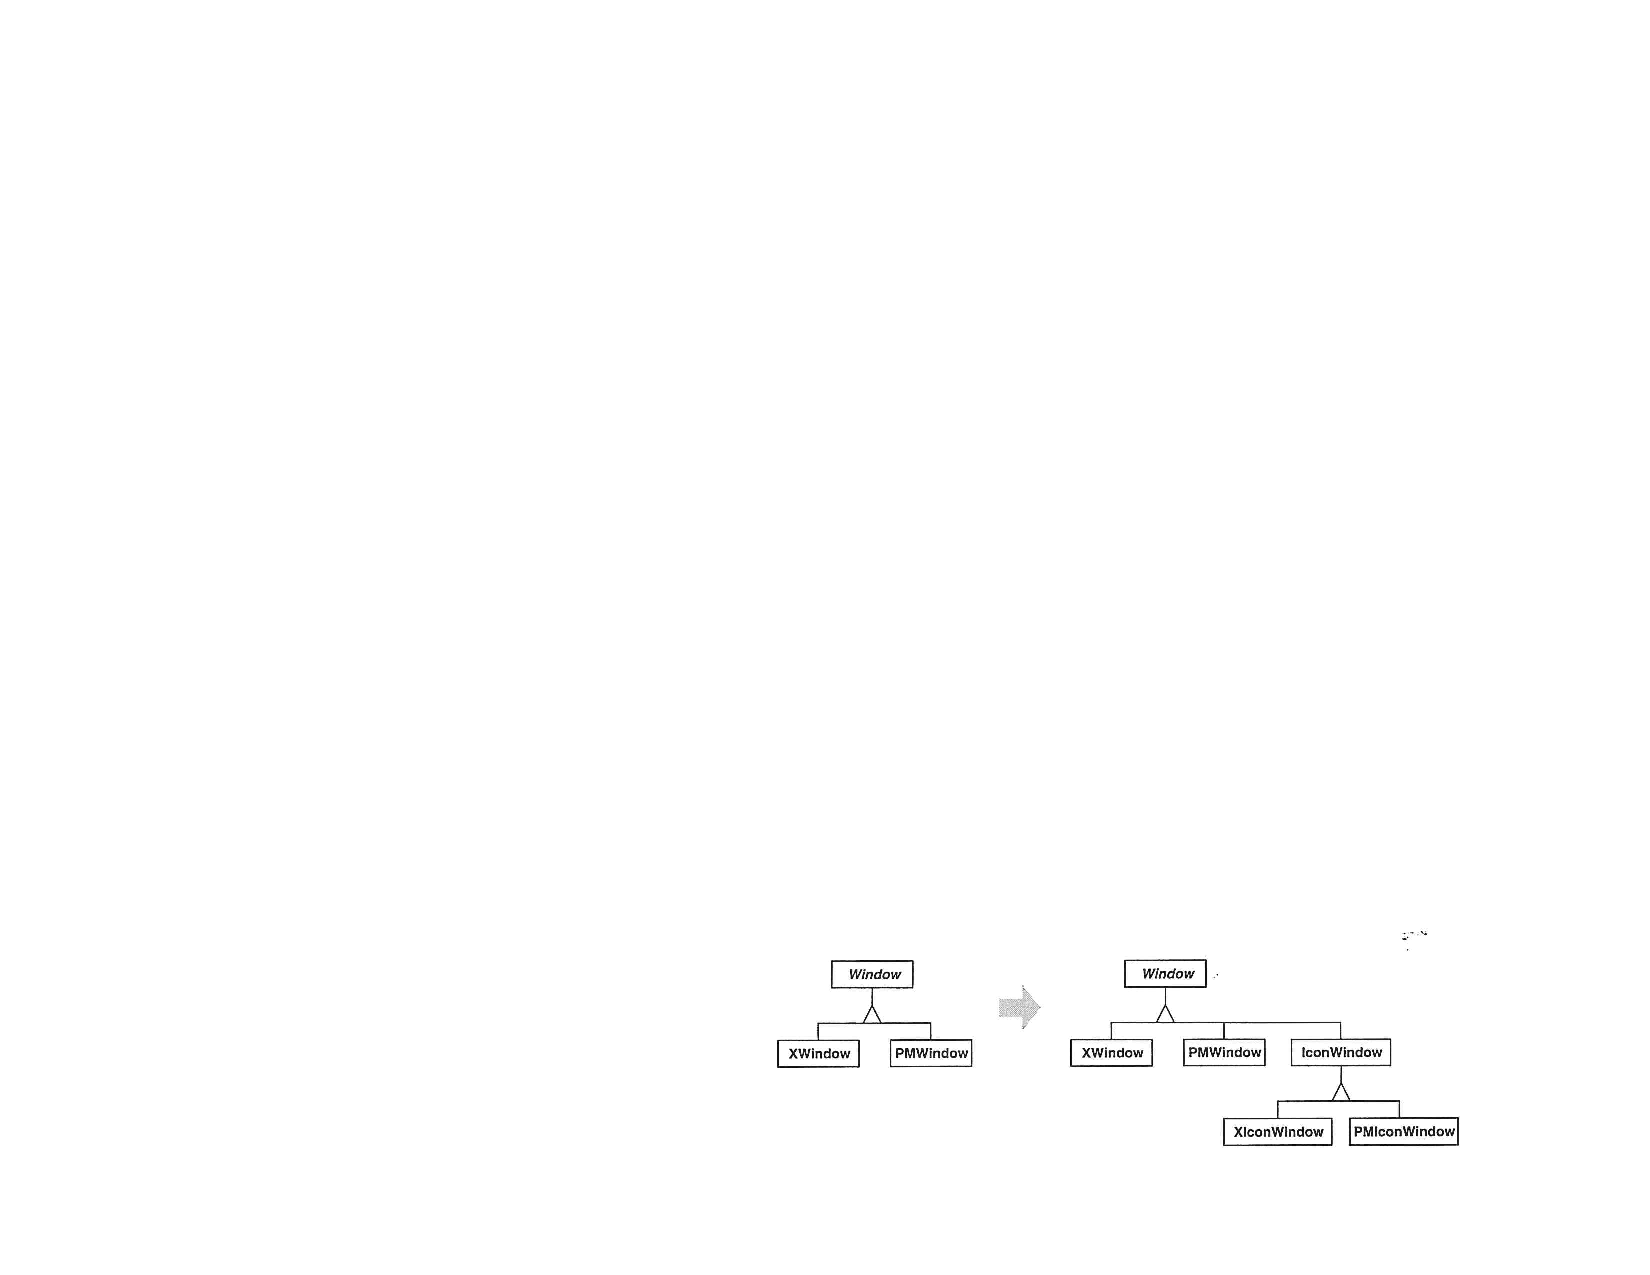
\includegraphics[width=0.6\textwidth]{bridge-1.pdf}
\caption{Bridge pattern: motivating example}
\end{figure}

Clients should be able to create a window without committing to a concrete implementation. 
Only the window implementation should depend on the platform on which the application runs. 
Therefore client code should instantiate windows without mentioning specific platforms. 

The Bridge pattern addresses these problems by putting the Window 
abstraction and its implementation in separate class hierarchies. 
\begin{itemize}
\item One class hierarchy for window interfaces 
(Window, IconWindow, TransientWindow) 
\item Separate hierarchy for platform-specific window implementations, with 
WindowImp as its root. The XWindowImp subclass, for example, provides an implementation based on the X Window 
System.
\end{itemize}

All operations on Window subclasses are implemented in terms of abstract operations from the 
WindowImp interface. This decouples the window abstractions from the various platform-specific 
implementations. We refer to the relationship between Window and WindowImp as a {\em bridge}, 
because it bridges the abstraction and its implementation, letting them vary independently.

\begin{figure}
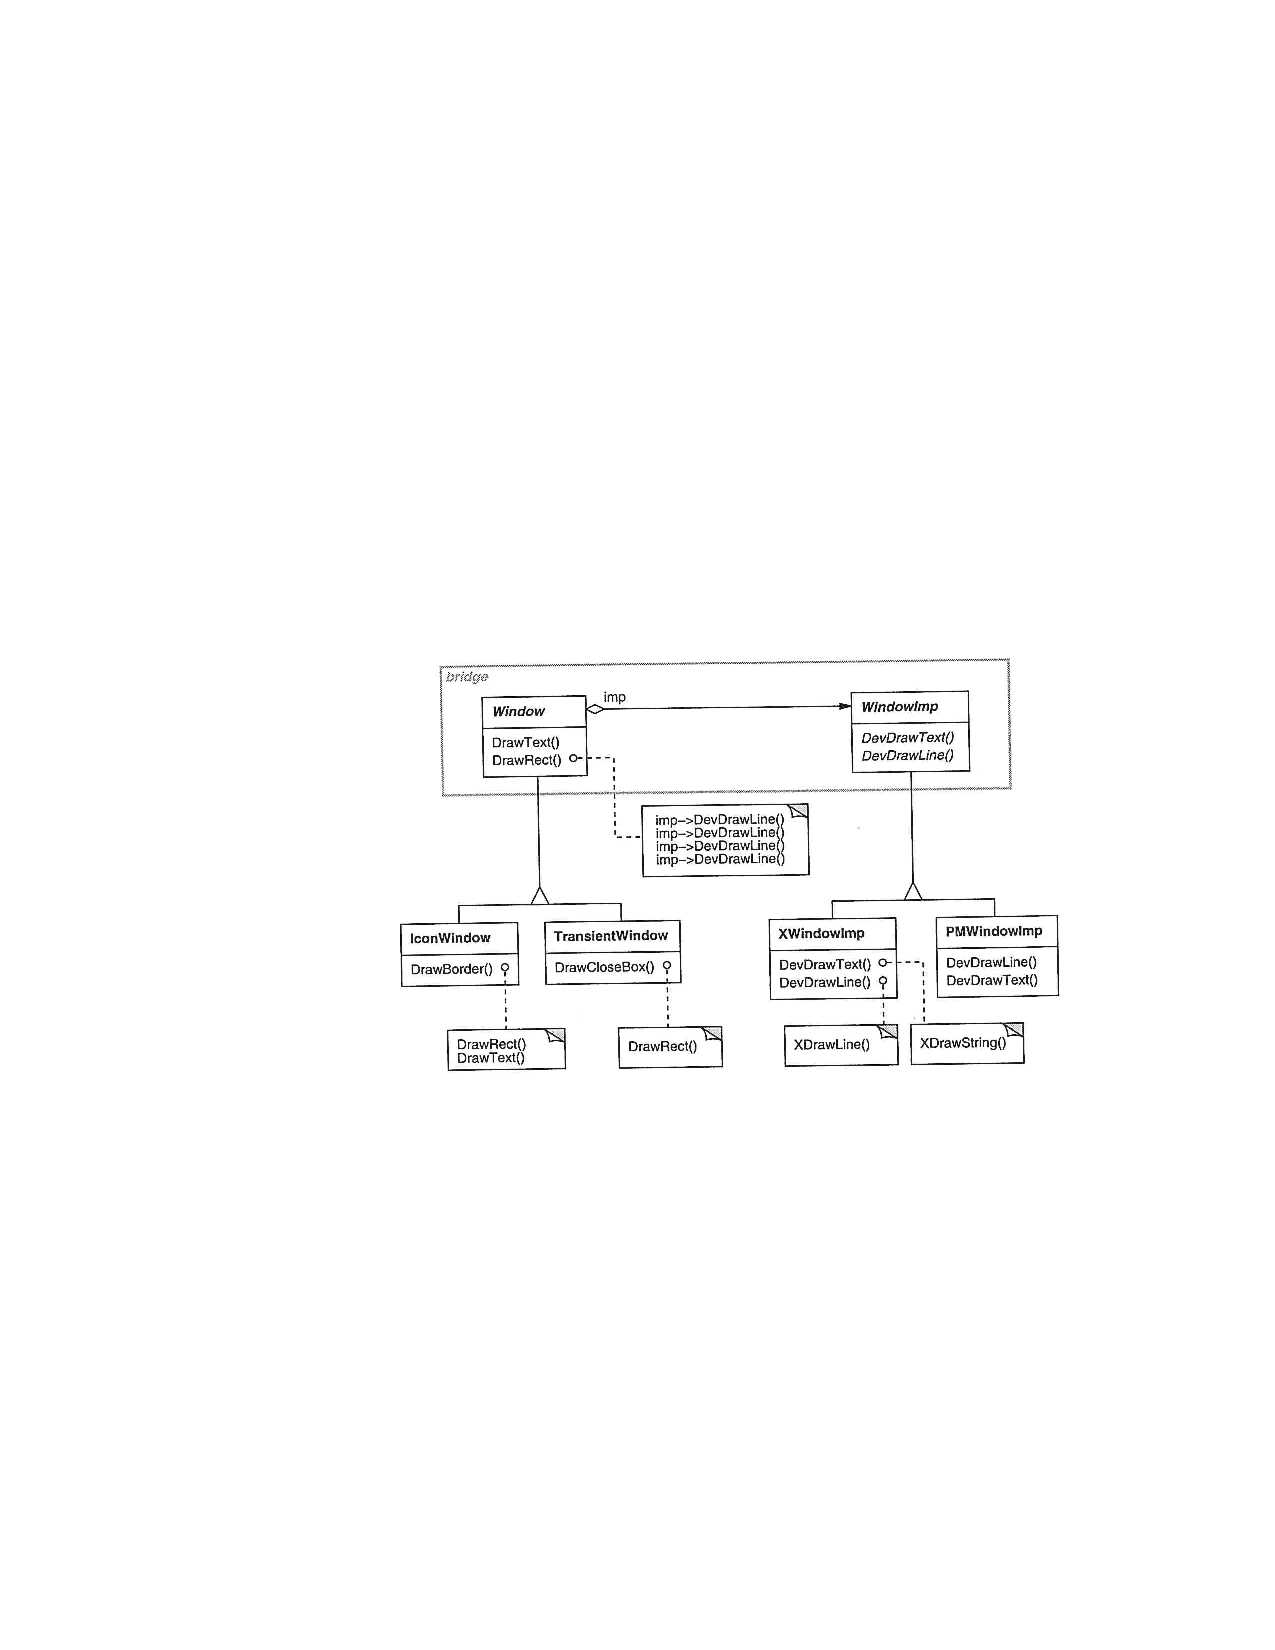
\includegraphics[width=0.8\textwidth]{bridge-2.pdf}
\caption{Bridge pattern applied to motivating example }
\end{figure}

\subsection{Code sketch}

Window interface:
\begin{lstlisting}
class Window {
   public:
     Window(View* contents);
     // requests handled by window
     virtual void DrawContents();
     virtual void Open();
     virtual void Close();
     virtual void Iconify();
     virtual void Deiconify();
     // requests forwarded to implementation
     virtual void SetOrigin(const Point& at);
     virtual void SetExtent(const Point& extent);
     virtual void Raise();
     virtual void Lower();
     virtual void DrawLine(const Point&, const Point&);
     virtual void DrawRect(const Point&, const Point&);
     virtual void DrawPolygon(const Point[], int n);
     virtual void DrawText(const char*, const Point&);
   protected:
     WindowImp* GetWindowImp();
     View* GetView();
   private:
     WindowImp* _imp;
     View* _contents; // the window's contents
   };
\end{lstlisting}

Window implementation:
\begin{lstlisting}
class WindowImp {
   public:
     virtual void ImpTop() = 0;
     virtual void ImpBottom() = 0;
     virtual void ImpSetExtent(const Point&) = 0;
     virtual void ImpSetOrigin(const Point&) = 0;
     virtual void DeviceRect(Coord, Coord, Coord, Coord) = 0;
     virtual void DeviceText(const char*, Coord, Coord) = 0;
     virtual void DeviceBitmap(const char*, Coord, Coord) = 0;
     // lots more functions for drawing on windows...
   protected:
     WindowImp();
};
\end{lstlisting}

For example, ApplicationWindow will implement DrawContents to draw the View instance it stores:
\begin{lstlisting}
   class ApplicationWindow : public Window {
   public:
     // ...
     virtual void DrawContents();
   };
   void ApplicationWindow::DrawContents () {
     GetView()->DrawOn(this);
}
\end{lstlisting}

IconWindow stores the name of a bitmap for the icon it displays...
\begin{lstlisting}
   class IconWindow : public Window {
   public:// ...
     virtual void DrawContents();
   private:
     const char* _bitmapName;
   };
\end{lstlisting}

It implements DrawContents to draw the bitmap on the window:
\begin{lstlisting}
void IconWindow::DrawContents() {
  WindowImp* imp = GetWindowImp();
    if (imp != 0) {
      imp->DeviceBitmap(_bitmapName, 0.0, 0.0);
    }
}
\end{lstlisting}

DrawRect implementation:
\begin{lstlisting}
void Window::DrawRect (const Point& p1, const Point& p2) {
  WindowImp* imp = GetWindowImp();
  imp->DeviceRect(p1.X(), p1.Y(), p2.X(), p2.Y());
}
\end{lstlisting}

X11 implementation:
\begin{lstlisting}
class XWindowImp : public WindowImp {
  public:
    XWindowImp();
    virtual void DeviceRect(Coord, Coord, Coord, Coord);
    // remainder of public interface...
  private:
    // lots of X window system-specific state, including: Display* _dpy;
    Drawable _winid; // window id
    GC _gc; // window graphic context 
};
\end{lstlisting}

PM implementation:
\begin{lstlisting}
class PMWindowImp : public WindowImp {
  public:
    PMWindowImp();
    virtual void DeviceRect(Coord, Coord, Coord, Coord);
    // remainder of public interface...
  private:
    // lots of PM window system-specific state, including:
    HPS _hps; 
};
\end{lstlisting}

DeviceRect implemented using X Window primitives:
\begin{lstlisting}
void XWindowImp::DeviceRect (
  Coord x0, Coord y0, Coord x1, Coord y1) {
    int x = round(min(x0, x1));
    int y = round(min(y0, y1));
    int w = round(abs(x0 - x1));
    int h = round(abs(y0 - y1)); XDrawRectangle(_dpy, _winid, _gc, x, y, w, h);
}
\end{lstlisting}

\section{Decorator}

\noindent{\em Intent:}
Attach additional responsibilities to an object dynamically. Decorators provide 
a flexible alternative to subclassing for extending functionality.

Sometimes we want to add responsibilities to individual objects, not to an entire class. 
A graphical user interface toolkit, for example, should let you add properties like 
borders or behaviors like scrolling to any user interface component.

One way to add responsibilities is with inheritance. Inheriting a border from another 
class puts a border around every subclass instance. This is inflexible, however, because the choice of border is made statically. A client can't control how and when to decorate the component with a border.

A more flexible approach is to enclose the component in another object that adds the border. 
The enclosing object is called a decorator. The decorator conforms to the interface of the component 
it decorates so that its presence is transparent to the component's clients. 
The decorator forwards requests to the component and may perform additional actions 
(such as drawing a border) before or after forwarding. 
Transparency lets you nest decorators recursively, thereby allowing an unlimited number of added responsibilities.

\begin{figure}
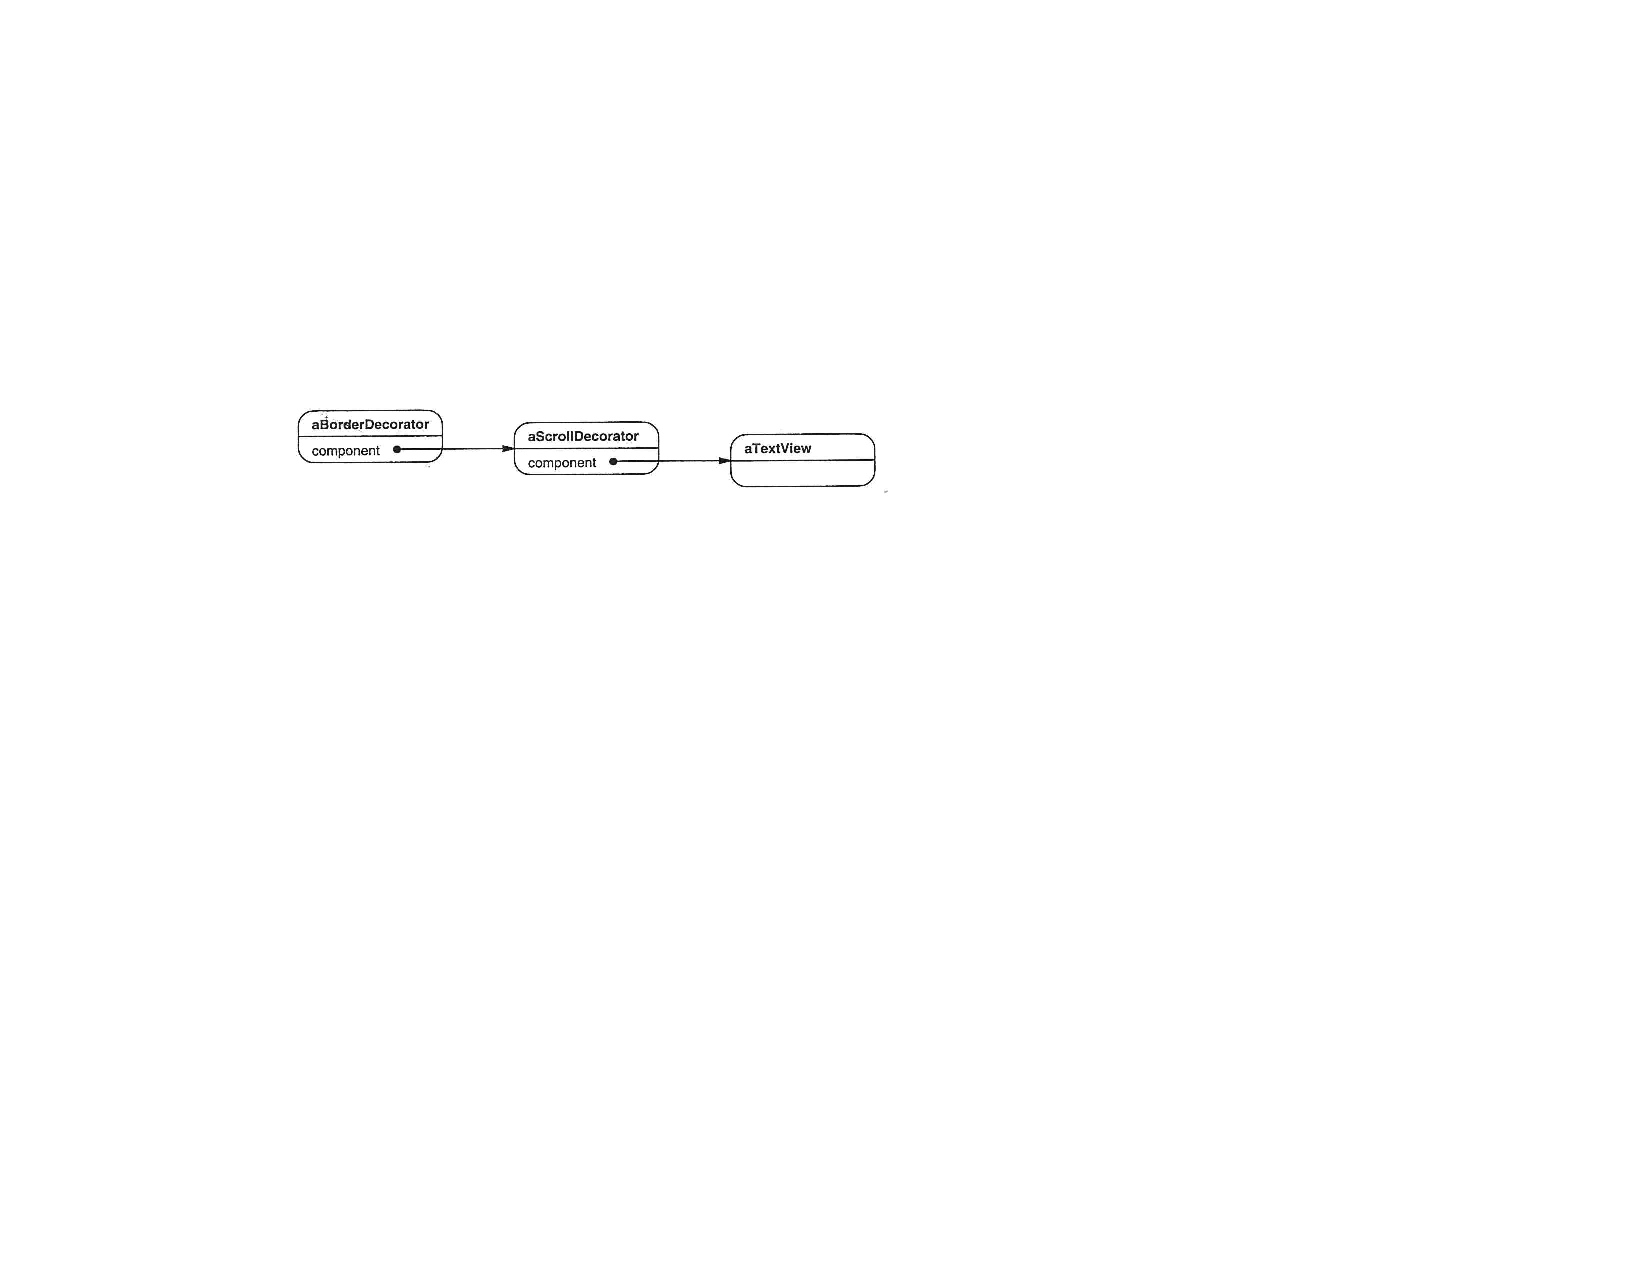
\includegraphics[width=0.6\textwidth]{deco-1.pdf}
\caption{Decorator pattern overview}
\end{figure}

\begin{figure}
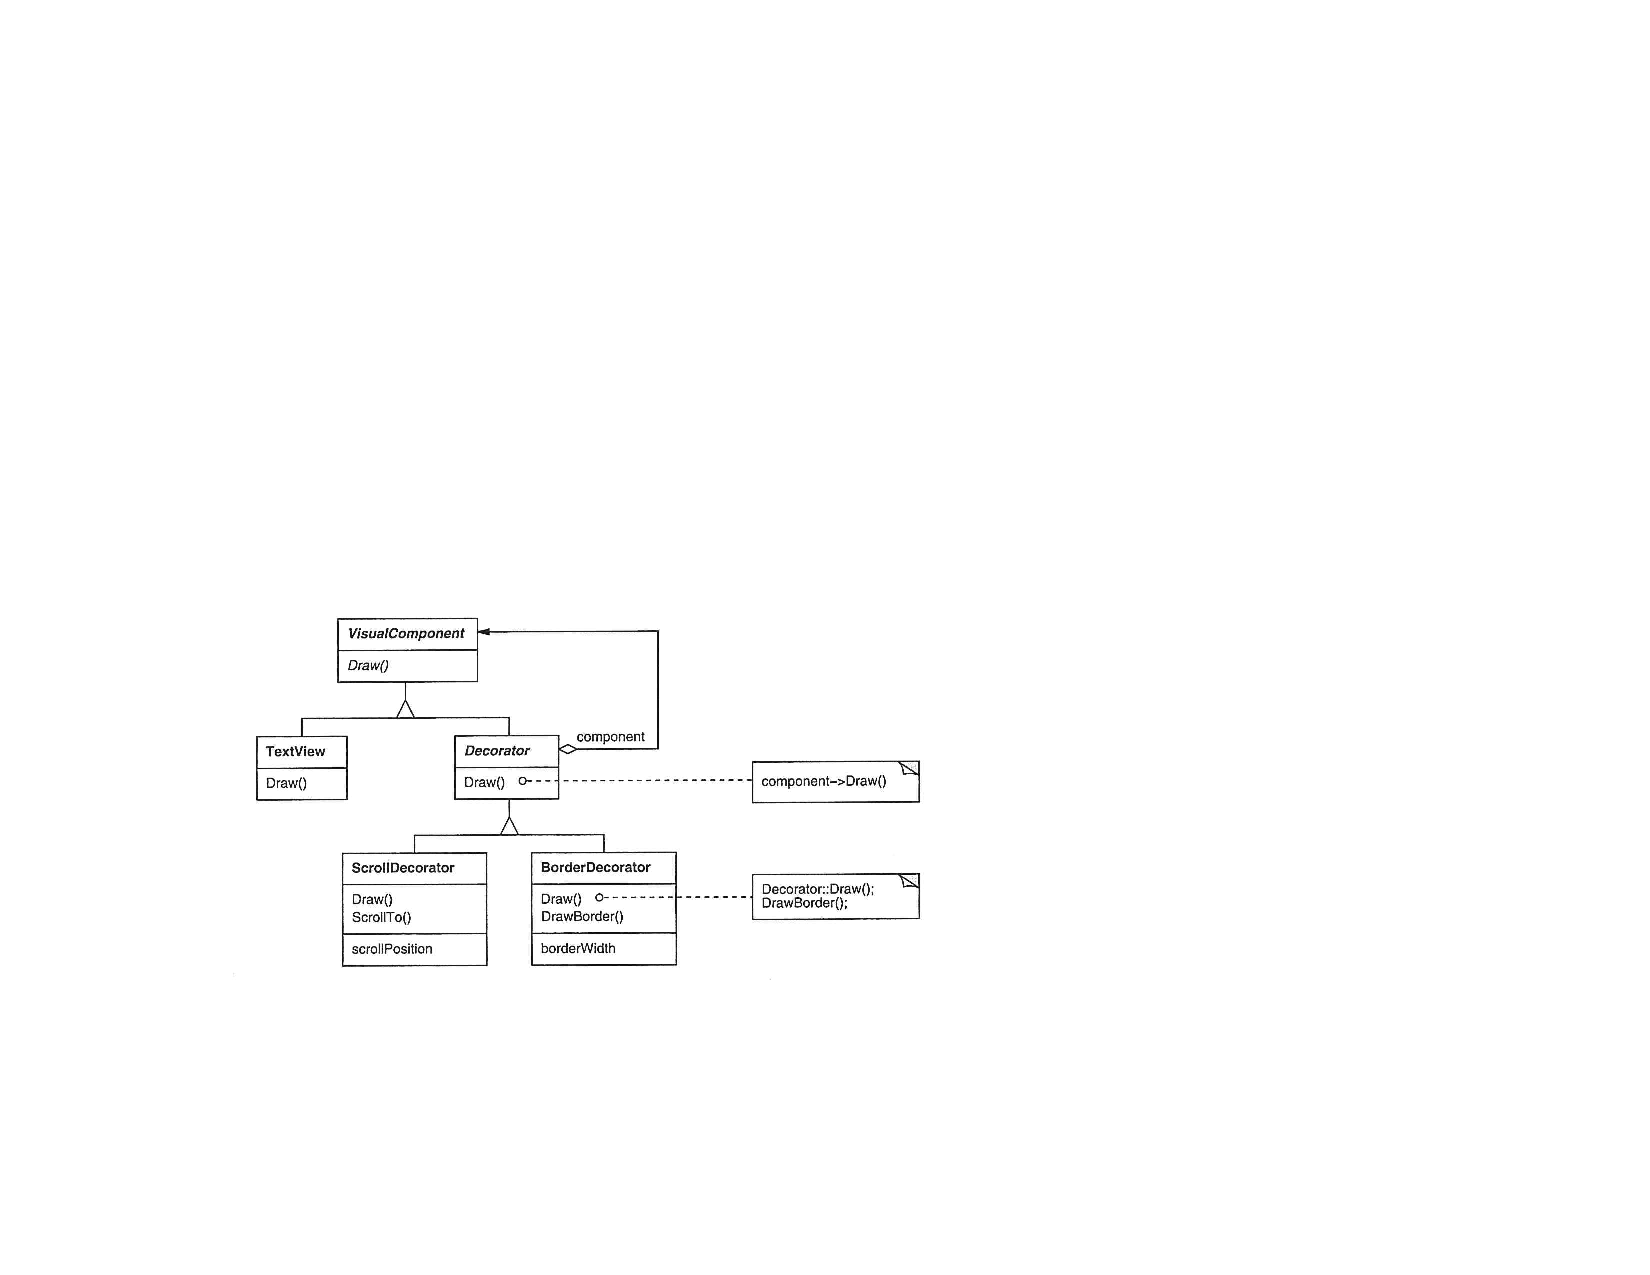
\includegraphics[width=0.8\textwidth]{deco-2.pdf}
\caption{Decorator pattern applied to motivating example }
\end{figure}

VisualComponent class:
\begin{lstlisting}
class VisualComponent {
  public:
    VisualComponent();
  virtual void Draw();
    virtual void Resize();
    // ...
};
\end{lstlisting}

Define a subclass of VisualComponent called Decorator, which is subclassed to obtain different decorations:
\begin{lstlisting}
   class Decorator : public VisualComponent {
   public:
       Decorator(VisualComponent*);
       virtual void Draw();
       virtual void Resize();
       // ...
   private:
       VisualComponent* _component;
};
\end{lstlisting}

For each operation in VisualComponent's interface, Decorator defines 
a default implementation that passes the request on to \_component:
\begin{lstlisting}
void Decorator::Draw () {
  _component->Draw();
}
void Decorator::Resize () {
  _component->Resize();
}
\end{lstlisting}

Subclasses of Decorator define specific decorations:
\begin{lstlisting}
class BorderDecorator : public Decorator {
  public:
    BorderDecorator(VisualComponent*, int borderWidth);
    virtual void Draw();
  private:
    void DrawBorder(int);
  private:
    int _width;
};

void BorderDecorator::Draw () {
  Decorator::Draw();
  DrawBorder(_width);
}
\end{lstlisting}

Assume Window class provides a SetContents operation to put a visual component into a window object:
\begin{lstlisting}
void Window::SetContents (VisualComponent* contents) {
  // ...
}
\end{lstlisting}

Now we can create the text view and a window to put it in:
\begin{lstlisting}
Window* window = new Window;
TextView* textView = new TextView;
\end{lstlisting}

TextView is a VisualComponent, which lets us put it into the window:
\begin{lstlisting}
window->SetContents(textView);
\end{lstlisting}
If we want a bordered and scrollable TextView we decorate it accordingly before putting it in the window.
\begin{lstlisting}
window->SetContents(
  new BorderDecorator(
    new ScrollDecorator(textView), 1
  )
);
\end{lstlisting}

Discussion:
\begin{itemize}
\item Decorator pattern provides more flexible way to add responsibilities to objects than can be had with 
inheritance. Responsibilities can be added and removed at run-time simply by 
attaching and detaching them. 

In contrast, inheritance requires creating a new class for each additional 
responsibility (e.g., BorderedScrollableTextView, BorderedTextView). This gives rise to many classes and increases 
the complexity of a system. Providing different Decorator classes for a specific Component class lets 
you mix and match responsibilities. 

Decorators also make it easy to add a property twice. For example, to give a 
TextView a double border, simply attach two BorderDecorators. Inheriting from a Border class twice is error-prone at 
best.

\item Avoids feature-laden classes high up in the hierarchy. Decorator offers a pay-as-you-go approach to adding 
responsibilities. 

Instead of trying to support all foreseeable features in a complex, customizable class, you can 
define a simple class and add functionality incrementally with Decorator objects. Functionality can be composed from 
simple pieces. As a result, an application needn't pay for features it doesn't use. It's also easy to define new 
kinds of Decorators independently from the classes of objects they extend, even for unforeseen extensions. Extending 
a complex class tends to expose details unrelated to the responsibilities you're adding.

\item A decorator and its component aren't identical. A decorator acts as a transparent enclosure. But from an 
object identity point of view, a decorated component is not identical to the component itself. Hence you shouldn't 
rely on object identity when you use decorators.

\item Lots of little objects. A design that uses Decorator often results in systems composed of lots of little 
objects that all look alike. The objects differ only in the way they are interconnected, not in their class or in 
the value of their variables. Although these systems are easy to customize by those who understand them, they can be 
hard to learn and debug.

\end{itemize}

Not limited to GUIs: Java I/O routines make heavy use of Decorators.

\section{Flyweight}

\noindent{\em Intent:}
Use sharing to support large numbers of fine-grained objects efficiently.

Motivation: Some applications could benefit from using objects throughout their design, but a naive implementation 
would be prohibitively expensive.

\begin{itemize}
\item Character objects in a text editor.
\item System for manipulating Boolean functions which uses Binary Decision Trees
to represent functions.
\end{itemize}

A flyweight is a shared object that can be used in multiple contexts simultaneously. The flyweight acts as an 
independent object in each context---it's indistinguishable from an instance of the object that's not shared. 
Flyweights cannot make assumptions about the context in which they operate. The key concept here is the distinction 
between intrinsic and extrinsic state. Intrinsic state is stored in the flyweight; it consists of information that's 
independent of the flyweight's context, thereby making it sharable. Extrinsic state depends on and varies with the 
flyweight's context and therefore can't be shared. Client objects are responsible for passing extrinsic state to the 
flyweight when it needs it.

For example, a document editor can create a flyweight for each letter of the alphabet. Each flyweight stores a character code, but its coordinate position in the document and its typographic style can be determined from the text layout algorithms and formatting commands in effect wherever the character appears. The character code is intrinsic state, while the other information is extrinsic.

Implementation: use a hash or an array of flyweight objects.

\chapter{Behavioral Patterns}

\section{Mediator}

\noindent{\em Intent:}
Define an object that encapsulates how a set of objects interact.
Mediator promotes loose coupling by keeping objects from referring to
each other explicitly, and it lets you vary their interaction independently.

Though partitioning a system into many objects generally enhances
reusability, proliferating interconnections tend to reduce it again.
Lots of interconnections make it less likely that an object can work
without the support of others---the system acts as though it were
monolithic. Moreover, it can be difficult to change the system's
behavior in any significant way, since behavior is distributed among
many objects.

Example: Consider the implementation of dialog boxes in a
graphical user interface. A dialog box uses a window to present a
collection of widgets such as buttons, menus, and entry fields.

Often there are dependencies between the widgets in the dialog. For example, 
a button gets disabled when a certain entry field is empty. Selecting an entry 
in a list of choices called a list box might change the contents of an entry field. 
Conversely, typing text into the entry field might automatically select one or more
corresponding entries in the list box. Once text appears in the entry field, 
other buttons may become enabled that let the user do something
with the text, such as changing or deleting the thing to which it refers.

You can avoid these problems by encapsulating collective behavior in a separate mediator object. 
A mediator is responsible for controlling and coordinating the interactions of a group of objects.
The mediator serves as an intermediary that keeps objects in the group
from referring to each other explicitly. 
The objects only know the mediator, thereby reducing the number of interconnections.
For example, FontDialogDirector can be the mediator between the widgets in a dialog box. 
A FontDialogDirector object knows
the widgets in a dialog and coordinates their interaction. 
It acts as a hub of communication for widgets.

Here's the succession of events by which a list box's selection passes to an entry field:
\begin{enumerate}
\item The list box tells its director that it's changed.
\item The director gets the selection from the list box.
\item The director passes the selection to the entry field.
\item Now that the entry field contains some text, the director enables button(s)
for initiating an action (e.g., "demibold," "oblique").
\end{enumerate}

\section{Observer}

\noindent{\em Intent:} 
Define a one-to-many dependency between objects so that when 
one object changes state, all its dependents are notified and updated
automatically.

Example: spreadsheet, histogram and pie chart view of data. 

\begin{lstlisting}
class Subject;
class Observer {
  public:
    virtual ~ Observer();
    virtual void Update(Subject* theChangedSubject) = 0;
  protected:
    Observer();
};
\end{lstlisting}

\begin{lstlisting}
class Subject {
  public:
    virtual ~Subject();
    virtual void Attach(Observer*);
    virtual void Detach(Observer*);
    virtual void Notify();
  protected:
    Subject();
  private:
    List<Observer*> *_observers;
};
\end{lstlisting}

See also Google Guava EventBus
\begin{verbatim}
http://code.google.com/p/guava-libraries/wiki/EventBusExplained
\end{verbatim}

\section{Strategy}
\noindent{\em Intent:}
Define a family of algorithms, encapsulate each one, and make them interchangeable. 
Strategy lets the algorithm vary independently from clients that use it.

Example: Many algorithms exist for breaking a stream of text into lines.
Hard-wiring all such algorithms into the classes that require them isn't desirable for several reasons:
\begin{itemize}
\item Clients that need linebreaking get more complex if they include
the linebreaking code. That makes clients bigger and harder to maintain, especially if they support multiple linebreaking algorithms.
\item Different algorithms will be appropriate at different times. We don't want to support multiple 
linebreaking algorithms if we don't use them all.
\item It's difficult to add new algorithms and vary existing ones when linebreaking is an integral part of a client.
\end{itemize}

We can avoid these problems by defining classes that encapsulate
different linebreaking algorithms. An algorithm that's 
encapsulated in this way is called a strategy.

\begin{itemize}
\item SimpleCompositor implements a simple strategy that determines linebreaks one at a time.
\item TeXCompositor implements the TeX algorithm for finding linebreaks. 
      This strategy tries to optimize linebreaks globally, that is, one paragraph at a time.
\item ArrayCompositor implements a strategy that selects breaks so that each row has a 
fixed number of items. 
\end{itemize}

Implementation: pass in strategy as function object (aka functor) or via template (limited to compile time selection).

\section{Visitor}

\noindent{\em Intent:} Represent an operation to be performed on the elements of an object
structure. Visitor lets you define a new operation without changing the
classes of the elements on which it operates.

Example: Consider a compiler that represents programs as abstract syntax trees.
It will need to perform operations on abstract syntax trees for ``static semantic'' analyses like 
checking that all variables are defined. It will also need to generate code. So it might define 
operations for type-checking, code optimization, flow analysis, checking for variables being assigned values before they're used, and so on. Moreover, we could use the abstract syntax trees for pretty-printing, 
program restructuring, code instrumentation, and computing various metrics of a program.

Most of these operations will need to treat nodes that represent assignment statements differently from nodes that 
represent variables or arithmetic expressions. Hence there will be one class for assignment
statements, another for variable accesses, another for arithmetic
expressions, and so on. 
The set of node classes depends on the language being compiled, of course, but it doesn't change much for a given
language.

This diagram shows part of the Node class hierarchy. The problem here
is that distributing all these operations across the various nodeclasses leads to a system that's hard to understand, maintain, and change. It will be confusing to have
type-checking code mixed with
pretty-printing code or flow analysis code. Moreover, adding a new
operation usually requires recompiling all of these classes. It would be better if each new operation 
could be added separately, and the node classes were independent of the operations that apply to them.

We can have both by packaging related operations from each class in a separate object, called a visitor, and passing it to elements of the abstract syntax tree as it's traversed. When an element ``accepts'' the visitor, it sends 
a request to the visitor that encodes the element's class. It also includes the element as an argument. 
The visitor will then execute the operation for that element---the operation that used to be in the class of the element.

With the Visitor pattern, you define two class hierarchies: one for the elements being operated on (the Node hierarchy) and one for the visitors that define operations on the elements (the NodeVisitor hierarchy). You create a 
new operation by adding a new subclass to the visitor class hierarchy. 
As long as the grammar that the compiler accepts doesn't change (that is, we don't 
have to add new Node subclasses), we can add new functionality simply by defining new NodeVisitor subclasses.

\end{document}
